%%%%%%%%%%%%%%%%%%%%%%%%%%%%%%%%%%%%%%%%%
% baposter Portrait Poster
% LaTeX Template
% Version 1.0 (15/5/13)
%
% Created by:
% Brian Amberg (baposter@brian-amberg.de)
%
% This template has been downloaded from:
% http://www.LaTeXTemplates.com
%
% License:
% CC BY-NC-SA 3.0 (http://creativecommons.org/licenses/by-nc-sa/3.0/)
%
%%%%%%%%%%%%%%%%%%%%%%%%%%%%%%%%%%%%%%%%%

%----------------------------------------------------------------------------------------
%	PACKAGES AND OTHER DOCUMENT CONFIGURATIONS
%----------------------------------------------------------------------------------------

\documentclass[portrait, a0paper, margin=7cm]{baposter}

\usepackage[font=small,labelfont=bf]{caption} % Required for specifying captions to tables and figures
\usepackage{booktabs} % Horizontal rules in tables
\usepackage{relsize} % Used for making text smaller in some places
\usepackage{helvet}
\usepackage{multicol}
\usepackage[export]{adjustbox}
\usepackage{float}

\graphicspath{{figures/}} % Directory in which figures are stored

\definecolor{bordercol}{RGB}{40,40,40} % Border color of content boxes
\definecolor{headercol1}{RGB}{190,212,180} % Background color for the header in the content boxes (left side)
\definecolor{headercol2}{RGB}{100,180,100} % Background color for the header in the content boxes (right side)
\definecolor{headerfontcol}{RGB}{40,1,1} % Text color for the header text in the content boxes
\definecolor{boxcolor}{RGB}{230,242,230} % Background color for the content in the content boxes
\definecolor{footcolor}{RGB}{255,255,255}

\begin{document}

%\background{ % Set the background to an image (background.pdf)
%	\begin{tikzpicture}[remember picture,overlay]
%	\draw (current page.north west)+(-2em,2em) node[anchor=north west]
%		{\includegraphics[height=1.1\textheight]{background}};
%	\end{tikzpicture}
%}

\begin{poster}{
grid=false,
columns=2,
headerheight=5cm,
borderColor=bordercol, % Border color of content boxes
headerColorOne=headercol1, % Background color for the header in the content boxes (left side)
headerColorTwo=headercol2, % Background color for the header in the content boxes (right side)
headerFontColor=headerfontcol, % Text color for the header text in the content boxes
boxColorOne=boxcolor, % Background color for the content in the content boxes
headershape=smallrounded, % Specify the rounded corner in the content box headers
headerfont=\Large\sf\bf\fontfamily{phv}\selectfont, % Font modifiers for the text in the content box headers
textborder=rectangle,
background=none,
headerborder=open, % Change to closed for a line under the content box headers
boxshade=plain
}
{}
%
%----------------------------------------------------------------------------------------
%	TITLE AND AUTHOR NAME
%----------------------------------------------------------------------------------------
%
{\sf\bf\fontfamily{phv}\selectfont Index Based Genome Mapper} % Poster title
	{\vspace{1em}\textbf{Maarja Lepamets and Fanny-Dhelia Pajuste}\\[0.4cm] % 		Author names
	{\smaller 
	Curriculum: Computer Science 2013/14\\	
	Institute of Computer Science\\
		Faculty of Mathematics and Computer Science\\
	 Tartu University\\[0.4cm]
	 Project repository: \Large \textit{https://github.com/maarjalepamets/read-mapping}}
} % Author email addresses
%
{
\includegraphics[scale=0.6]{ut}} % University/lab logo


%----------------------------------------------------------------------------------------
%	INTRODUCTION
%----------------------------------------------------------------------------------------


\headerbox{Introduction}{name=intr,column=0,row=0,span=1}{
\textbf{One of the "hottest" terms in today's medical world is "personal medicine". For this to be possible, scientists need to sequence as many individuals as possible and map the reads back to the reference genome to find out the locations of the given sub-sequences, expression rates of the genes or the sequence of the full genome. This kind of biological data is, however, so large that using several software applications in its analysis is inevitable. When it comes to indexing and mapping to the genome, there are two widely-used algorithmic approaches. One involves modifications of suffix trees and Burrows-Wheeler transformation, another different kinds of hashing (Schbath \textit{et al}, 2012). In this project we were implementing a latter type of genome indexer together with a mapping tool which relies on pairing every $n$-nucleotide sequence with its locations in a genome.}
}

\headerbox{Indexing the Genome}{name=ind,column=0,below=intr} {
The first step of mapping the sequencing reads is to index the full genome. For this we iterate over all chromosomes and extract each $n$-nucleotide ($n \le 16$) word together with its genomic location. Then we sort the words using a linear time in-place radix sort combined with insertion sort for small buckets (Duvanenko, 2009) and keep only one copy of each word and a pointer to the starting position of its genomic locations. The overall time-complexity of the algorithm is $O(n)$ and altogether it takes $4\ \times$ \textit{size of the genome} $+\ 8\ \times$ \textit{unique word in the genome} bytes. The measurements of run-time on four different organisms and two different word lengths are given in Table 1.

\begin{figure}[H]
\begin{center}
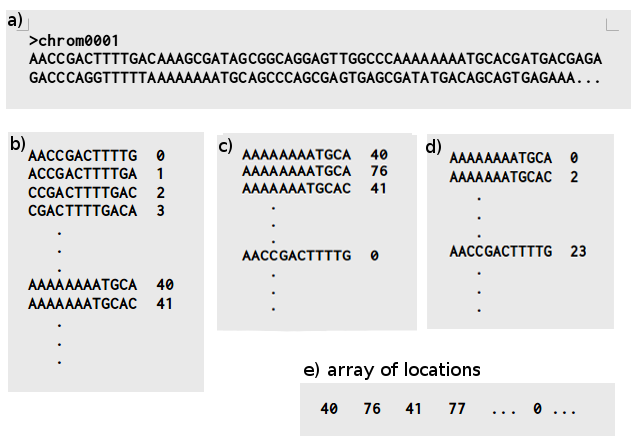
\includegraphics[scale=0.35]{radix}
\caption{\textbf{a)} Genome sequence; \textbf{b)} All extracted $n$-mers; \textbf{c)} $n$-mers sorted with in-place radix sort; \textbf{d)} Only one copy of each $n$-mer and the pointer to the array of locations (\textbf{e)}).}
\end{center}
\end{figure}

\begin{table}[H]
\begin{center}
\caption {Measurements of run-time} 

\begin{tabular}{ccc}
& $n = 10$ & $n = 16$\\
\hline
\textit{E. coli} & 0 min 0.5 s & 0 min 0.6 s\\
\hline
\textit{P. aeruginosa} & 0 min 0.7 s & 0 min 0.8 s\\
\hline
\textit{Mus musculus} & 16 min 22.1 s & 26 min 15.4 s\\
\hline
\textit{H. sapiens} & 18 min 26.8 s & 33 min 48.5 s\\
\end {tabular}
\end{center}
\end{table}

}



\headerbox{Mapping Tool}{name=map,column=1, row=0} {
The mapping process consists of two parts. In the first part the read is cut into over-lapping $n$-nucleotide seeds. The index created in the previous step is then used to find all locations of those seeds in the genome. When all seeds map to the similar location on the genome, we have found a perfect match. If only some map, we move to the second part of the mapping to find matches with errors by calculating simple edit distance between our read and the potential region in the genome. The time-complexity of the mapping tool is $O(m\log n)$ where $m$ is the number of words and $n$ the length of the genome.

\begin{figure}[H]
\begin{center}
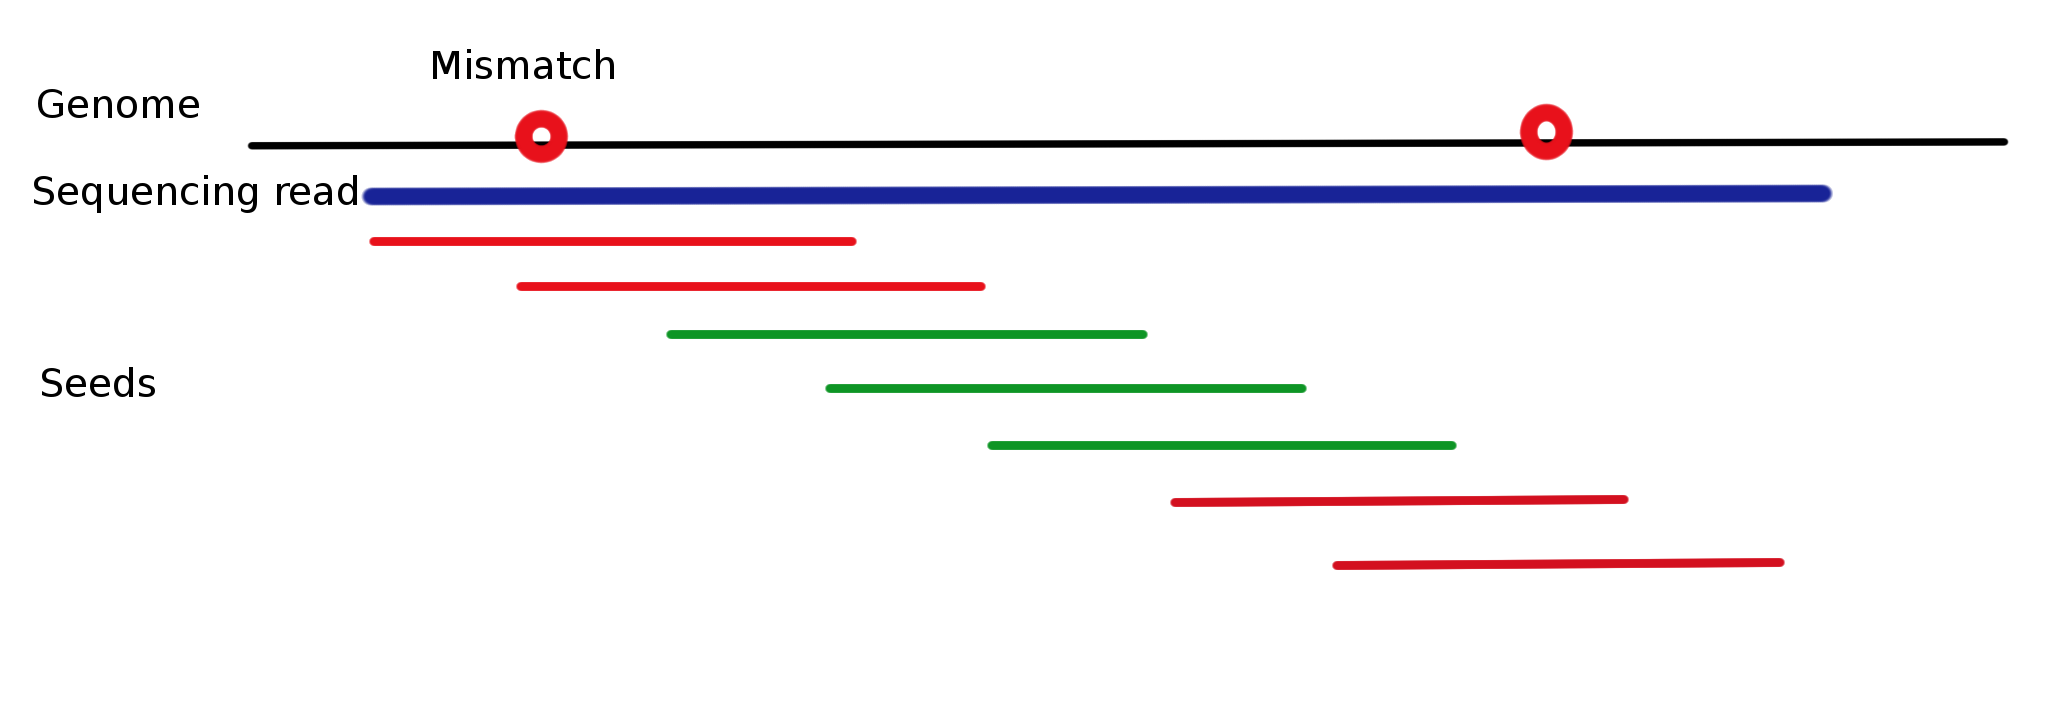
\includegraphics[scale=0.5]{map}
\caption{Read is cut into seeds. Green seeds map to the given genome location, red seeds do not because of the mismatches (red dots). The second part of the mapping tool is for deciding whether there are more or less mismatches in this genome region that what the user allows.}
\end{center}
\end{figure}

}

\headerbox{Validation}{name=res,column=1,below=map} {

}

\headerbox{References}{name=ref,column=1,below=res} {

\smaller % Reduce the font size in this block

Schbath, S., Martin, V., Zytnicki, M., Fayolle, J., Loux, V., Gibrat, J.-F. (2012) Mapping Reads on a Genomic Sequence: An Algorithmic Overview and a Practical Comparative Analysis. J Comput Biol., 19(6): 796-813.\\

Duvanenko, V. J. (2009) In-place Hybrid N-bit-Radix Sort. http://www.drdobbs.com/architecture-and-design/algorithm-improvement-through-performanc/221600153\\
}


\headerbox{}{name=footer, column=1, span=1, above=bottom, below=ref, textborder=none,headerborder=none,boxheaderheight=0pt, boxColorOne = footcolor}{

\begin{tabular}{p{2cm} p{2cm} p{5cm}}

& 
\includegraphics[scale=0.35]{ati}  & {
\includegraphics[scale=0.35]{it}}

\end{tabular}
 
}


\end{poster}

\end{document}